\documentclass[9pt, handout]{beamer}
\usetheme{CambridgeUS}
\usepackage{xcolor}
\usepackage{geometry}
\usepackage{array}
\usepackage{comment}

\AtBeginSection[]
{
  \begin{frame}
    \frametitle{Table of Contents}
    \tableofcontents[currentsection]
  \end{frame}
}

\setbeamertemplate{footline}
{
  \leavevmode%
  \hbox{%
    \begin{beamercolorbox}[wd=.333333\paperwidth,ht=2.25ex,dp=1ex,center]{author in head/foot}%
      \usebeamerfont{author in head/foot}\insertshortauthor
    \end{beamercolorbox}%
    \begin{beamercolorbox}[wd=.333333\paperwidth,ht=2.25ex,dp=1ex,center]{title in head/foot}%
      \usebeamerfont{title in head/foot}\insertshortsubtitle
    \end{beamercolorbox}%
    \begin{beamercolorbox}[wd=.333333\paperwidth,ht=2.25ex,dp=1ex,right]{date in head/foot}%
      \usebeamerfont{date in head/foot}\insertshortdate{}\hspace*{2em}
      \usebeamertemplate{page number in head/foot}\hspace*{2ex}
    \end{beamercolorbox}
  }%
  \vskip0pt%
}

\title{Principles of Economics}
\subtitle{Discussion Session 1}
\author{Joe Wilske and Yuzhi Yao}
\institute{Boston College}
\date{\today}

\begin{document}

\frame{\titlepage}

\begin{frame}{Shift `of' a curve \textit{vs} shift `along' a curve}
    \begin{itemize}
        \item A demand curve is a function $Q^D(P)$.\\
        \begin{itemize}
            \item Input a price and it returns the quantity demanded.
            \vspace{5}
        \end{itemize}
        \item Changing the input from $P_1$ to $P_2$ implies shifting between two points on the \textit{same curve}:\\
        $(P_1, Q^D(P_1)) \: \longrightarrow \: (P_2, Q^D(P_2))$.
        \vspace{5}
        \item Changing other parameters of the function besides $P$ implies shifting the \textit{curve itself}:\\
        $Q_1^D \: \longrightarrow \: Q_2^D$
    \end{itemize}
    \vspace{20}
    What might those other parameters be for a demand curve? A supply curve?
\end{frame}

\begin{frame}{Exercise 1: Demand \& Supply Curves}
    Q1: Draw a demand curve for orange juice, $D_1$, and choose a point $A(Q_1, P_1)$ on the demand curve. What happens in the following scenarios?  Why?
    \begin{itemize}
        \item[-] Price of apple juice rises
        \item[-] Price of orange juice falls
    \end{itemize}
    \vspace{0.1in}
    Q2: Draw a supply curve for apple juice, $S_1$, and choose a point $B(Q_1, P_1)$ on the supply curve. What happens to it in each of the following scenarios? Why? 
    \begin{itemize}
        \item[-] Grocery stores cut the price of apple juice
        \item[-] A technological advance allows apple juice to be produced at a lower cost
    \end{itemize}
    \vspace{1.5in}
\end{frame}

\begin{frame}{Exercise 1: Demand \& Supply Curves}
    \begin{figure}
        \centering
        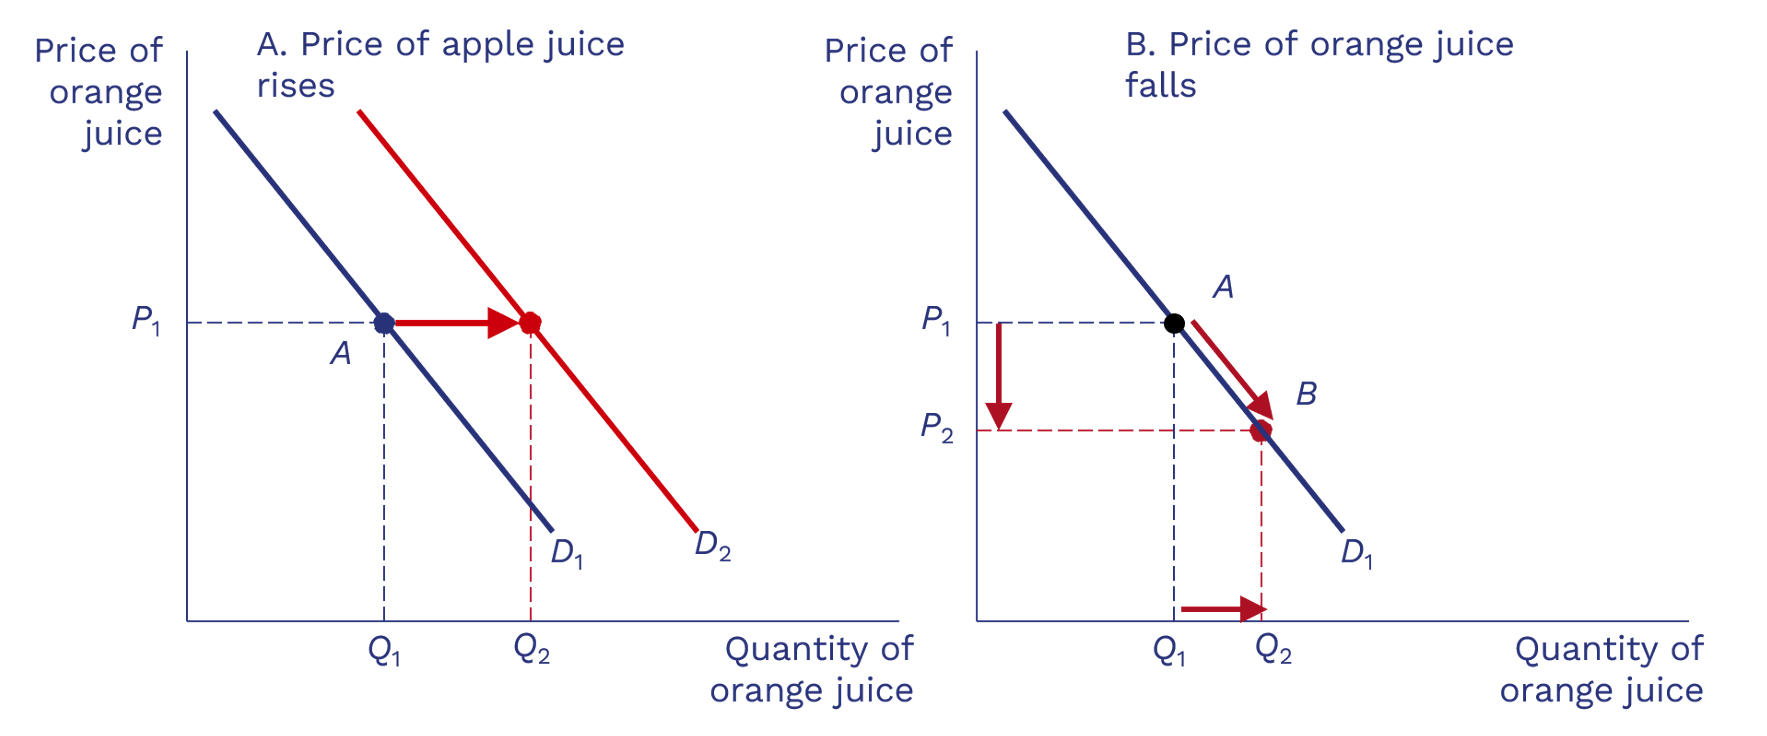
\includegraphics[width=0.9\linewidth]{fig1.png}
        \caption{Solution for Q1}
    \end{figure}
\end{frame}

\begin{frame}{Exercise 1: Demand \& Supply Curves}
    \begin{figure}
        \centering
        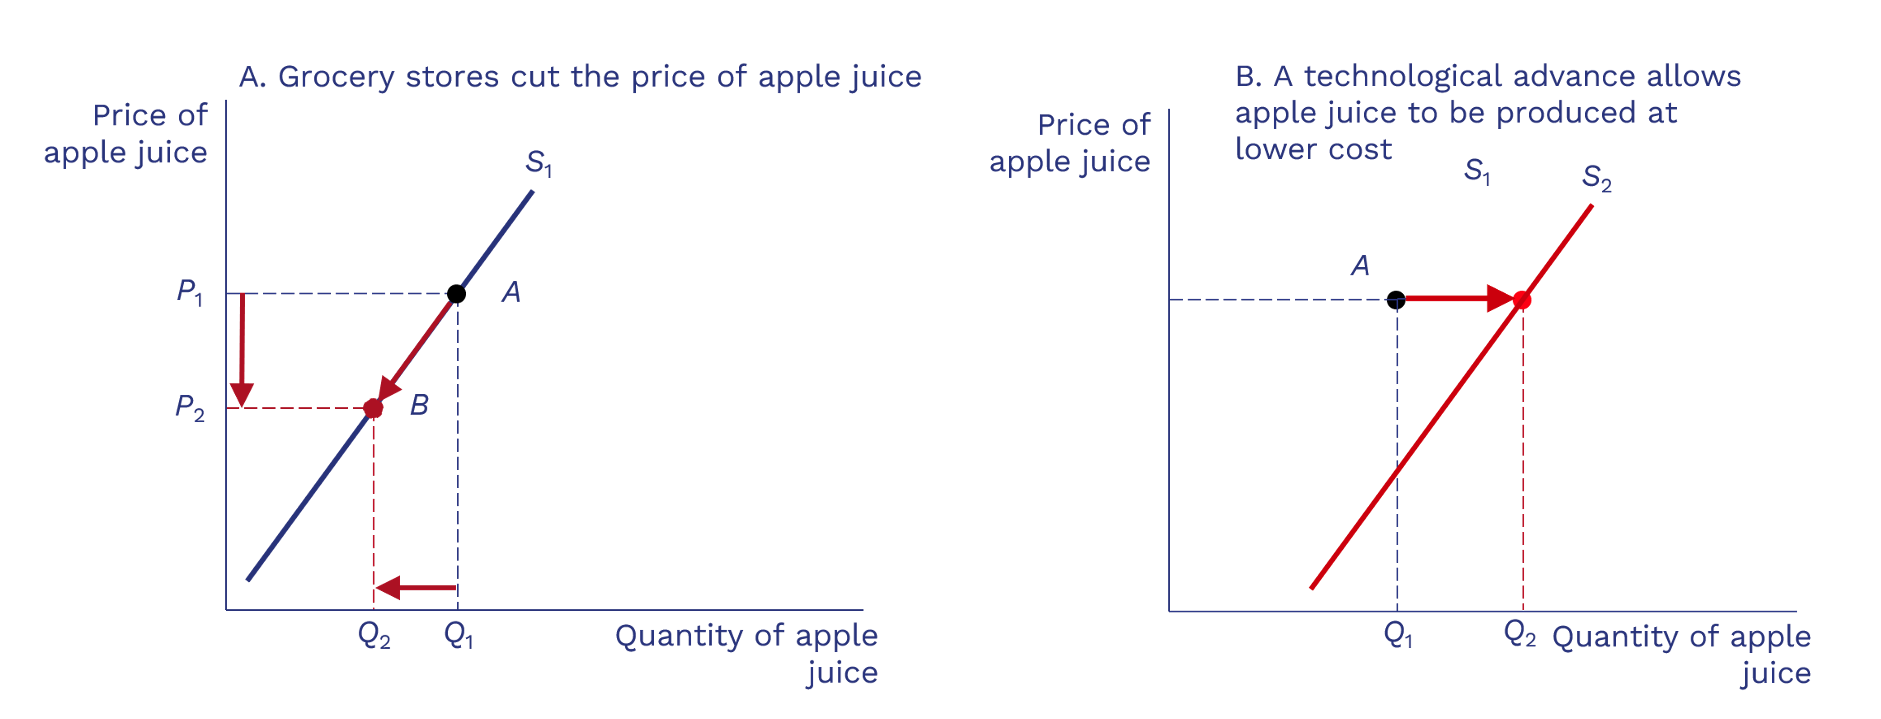
\includegraphics[width=0.9\linewidth]{fig2.png}
        \caption{Solution for Q2}
    \end{figure}
\end{frame}

\begin{frame}{Exercise 2: Shifts in Supply and Demand}
    The \textbf{three-step method}: an ``econ 101" technique for market analysis
    \begin{enumerate}
        \item Identify which curve is effected (D or S)
        \item Decide which direction it shifts (and shift it)
        \item Find new equilibrium price and quantity
    \end{enumerate}
    \vspace{25}
    Use the three-step method to analyze the effects of these events on the equilibrium price and quantity of orange juice
    \begin{itemize}
        \item[-] There is a fall in the price of apple juice
        \item[-] Good weather creates an abundant orange crop
        \item[-] Both events occur simultaneously
    \end{itemize}
    \vspace{2in}
\end{frame}

\begin{frame}{Exercise 2: Shifts in Supply and Demand}
    \begin{figure}
        \centering
        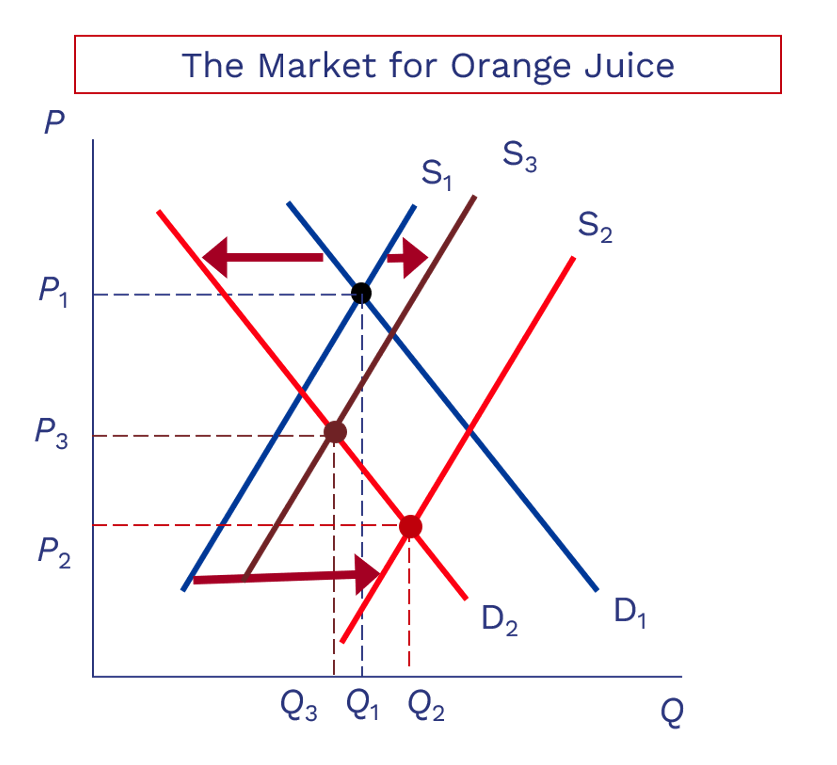
\includegraphics[width=0.5\linewidth]{fig3.png}
        \caption{Solution for Q3}
    \end{figure}
\end{frame}

\begin{frame}{Exercise 3: Solve Equilibrium Numerically}
    Suppose the demand and supply of coffee are given by:
    \begin{itemize}
        \item[-] $Q^D=20 - 2P$ 
        \item[-] $Q^S = 4P - 4$
    \end{itemize}
    Q1: Draw the demand and supply curves;\\
    Q2: Solve for the equilibrium price and quantity;\\
    Q3: Suppose the market price changes to \$7. Solve for $Q^D$ and $Q^S$.
    \vspace{2in}
\end{frame}

\begin{frame}{Exercise 3: Solve Equilibrium Numerically}
    Solution:
    \begin{enumerate}
        \item (draw)
        \item $P^*=4$, $Q^*=12$
        \item $Q^D=6$, $Q^S=24$
    \end{enumerate}
\end{frame}
\end{document}

